\documentclass{article}
\setlength\parindent{0pt}
\setlength{\parskip}{0.3cm}
\usepackage{color}
\usepackage{graphicx}
\usepackage{subfigure}
\usepackage{multirow}
\usepackage{miller}
\usepackage{amsmath}
\usepackage{pbox}
\usepackage{hyperref}
\usepackage{fancyvrb}
\usepackage{environ}
\usepackage{verbatim}
\usepackage{lscape}
%\usepackage{tikz}
\usepackage[a4paper,bindingoffset=0.2in,left=1in,right=1in,top=1in,bottom=1in,footskip=.25in]{geometry}

%\makeatletter
%\DeclareRobustCommand*{\escapeus}[1]{%
%  \begingroup\@activeus\scantokens{#1\endinput}\endgroup}
%\begingroup\lccode`\~=`\_\relax
%   \lowercase{\endgroup\def\@activeus{\catcode`\_=\active \let~\_}}
%\makeatother

\newcommand{\escapeus}[1]{\verb|#1|}



\definecolor{deepblue}{rgb}{0,0,0.5}
\definecolor{deepred}{rgb}{0.6,0,0}
\definecolor{deepgreen}{rgb}{0,0.5,0}

\usepackage{listings}
%\usepackage{xcolor}
%\usepackage{minted}

\DeclareFixedFont{\ttb}{T1}{txtt}{bx}{n}{10} % for bold
\DeclareFixedFont{\ttm}{T1}{txtt}{m}{n}{10}  % for normal
\DeclareFixedFont{\tti}{T1}{txtt}{m}{it}{10}  % for italic

\newcommand{\vect}[1]{\boldsymbol{\mathrm{#1}}}
\let\stdsection\section
\renewcommand\section{\pagebreak\stdsection}

\newcommand{\nanocap}{\texttt{NanoCap}}
\newcommand{\python}{\texttt{Python}}
\renewcommand{\lstlistingname}{NanoCap Code}

\definecolor{mygreen}{rgb}{0,0.6,0}
\definecolor{mygray}{rgb}{0.5,0.5,0.5}
\definecolor{mymauve}{rgb}{0.58,0,0.82}
\definecolor{myterminalbg}{rgb}{0.1,0.1,0.1}
\definecolor{mycodebg}{rgb}{1, 0.973, 0.89}
\definecolor{myterminalfont}{rgb}{0.95,0.95,0.95}
\definecolor{mycodeborder}{rgb}{0.89, 0.89, 0.89}


\title{NanoCap Guide \& Documentation}
\date{}
\begin{document}
%\maketitle
\begin{figure}[h!]
\centering

\includegraphics[scale= 1.0]{../../../../logos/nanocap_logo_medium.png}
\end{figure}
\begin{center}\large\textbf{Guide \& Documentation}\end{center}
\begin{center}\normalsize\textbf{M. Robinson }\end{center}
\begin{center}\small\textbf{2012-2014}\end{center}
%\begin{center}\tiny\textbf{Copyright (c) 2012-2014}\end{center}
\normalsize{}



\nanocap~provides both libraries and a standalone application for the construction 
of capped nanotubes of arbitrarily chirality and fullerenes of any radius. Structures 
are generated by constructing a set of optimal dual graph topologies which 
are subsequently optimised using a carbon interatomic potential. Combining 
this approach with a GUI featuring 3D rendering capabilities allows for the rapid 
inspection of physically sensible structures which can be used as input for 
molecular simulation.

The \nanocap~source and builds for different platforms can be found at:

\href{http://sourceforge.net/projects/nanocap/}{\texttt{http://sourceforge.net/projects/nanocap/}}

The \nanocap~documentation is outlined in the following sections.

\tableofcontents




\section{Installation}

There are three approaches to using \nanocap:

\begin{enumerate}
 \item As a standalone application.
 \item From source without rendering/GUI capabilities
 \item From source with rendering/GUI capabilities
\end{enumerate}

The installation procedures involved in each of the options above vary with increasing complexity yet this is balanced with an increase in versatility. For example, \nanocap~ compiled from source with with rendering and GUI capabilities can be used in parallelised code to produce and visualise multiple structures.


\subsection{Requirements}

\begin{enumerate}

\item As a standalone application.
 
\nanocap~ is built into a DMG for OSX and a .EXE for Windows. The required libraries listed below are bundled but not modified in line with the associated licenses. 

\textbf{OSX}:  \nanocap~works \textit{straight out of the box} simply extract the application from the DMG and drag it into the \textbf{Applications} folder.

\textbf{Windows}:  \nanocap~requires the Microsoft Visual C++ 2008 Redistributable Package which can be obtained from:

 \url{http://www.microsoft.com/en-au/download/details.aspx?id=29}


 \item From source without rendering/GUI capabilities

\begin{itemize}
 \item NumPy - Version 1.6.2
 \item Scipy - Version 0.11.0
 \item sqlite3 Version 2.6.0 (bundled with Python)
 \item C compiler (e.g. GCC)
 \item Fortran compiler (e.g. GFortran)
 \end{itemize}
 
 \item From source with rendering/GUI capabilities

\begin{itemize}
 \item Qt - Version 4.8.5 
 \item PySide - Version 1.1.1 (depends on Qt)
 \item VTK - Version 5.8 (+ Python Wrappers)
 \end{itemize}
 
 \end{enumerate}
Installation of the dependencies above is platform dependent and there are multiple methods of achieving the required python working environment. The simplest options are using package managers or binary distributions, i.e:
\newline\newline
OSX:
\begin{itemize}
 \item Homebrew \url{http://brew.sh}
 \item MacPorts \url{http://www.macports.org}
 \item Fink \url{http://www.finkproject.org/}
 \end{itemize}
Windows:
\begin{itemize}
 \item PythonXY \url{http://code.google.com/p/pythonxy}
 \item Enthought Python \url{http://www.enthought.com/products/epd}
 \end{itemize}
 Linux:
 \begin{itemize}
\item apt-get 
\item YUM (RPM Package Manager)
 \end{itemize}
 
\subsection{Installing from source}

After obtaining and installing the previously outlined requirements, a tar ball of \nanocap~can be downloaded from:

\url{http://sourceforge.net/projects/nanocap/files/src/}

As an alternative, the latest release can be checked out from the \texttt{mercurial} repository:
\begin{lstlisting}[keywordstyle={\color{myterminalfont}},
			language={sh},
			commentstyle={\it\color{myterminalfont}},
			emphstyle={\ttb\color{myterminalfont}},
			stringstyle={\color{myterminalfont}},
			showstringspaces={false},
			otherkeywords={self},
			emph={MyClass,__init__},
			frame={},
			basicstyle={\ttm\color{myterminalfont}},
			morekeywords={True,False},
			captionpos={b},
			backgroundcolor={\color{myterminalbg}}]		
bash-3.2$ hg clone http://hg.code.sf.net/p/nanocap/code-0 nanocap-code-0
\end{lstlisting}
After download and unpacking (if required), installation proceeds in the typically python fashion:
\begin{lstlisting}[keywordstyle={\color{myterminalfont}},
			language={sh},
			commentstyle={\it\color{myterminalfont}},
			emphstyle={\ttb\color{myterminalfont}},
			stringstyle={\color{myterminalfont}},
			showstringspaces={false},
			otherkeywords={self},
			emph={MyClass,__init__},
			frame={},
			basicstyle={\ttm\color{myterminalfont}},
			morekeywords={True,False},
			captionpos={b},
			backgroundcolor={\color{myterminalbg}}]		
bash-3.2$ python setup.py install
\end{lstlisting}

The installation runs a configure script (generated by \texttt{autoconf}) that detects available C and Fortran compilers and builds the associated shared libraries. To test for a successful installation, simply attempt to import \nanocap~in a python terminal. 

\begin{lstlisting}[keywordstyle={\color{myterminalfont}},
			language={sh},
			commentstyle={\it\color{myterminalfont}},
			emphstyle={\ttb\color{myterminalfont}},
			stringstyle={\color{myterminalfont}},
			showstringspaces={false},
			otherkeywords={self},
			emph={MyClass,__init__},
			frame={},
			basicstyle={\ttm\color{myterminalfont}},
			morekeywords={True,False},
			captionpos={b},
			backgroundcolor={\color{myterminalbg}}]		
bash-3.2$ python
Python 2.7.3 (default, Jul 19 2012, 13:57:53) 
[GCC 4.2.1 Compatible Apple Clang 3.1 (tags/Apple/clang-318.0.61)] on darwin
Type "help", "copyright", "credits" or "license" for more information.
>>> import nanocap
>>> print nanocap.__version__
1.0b9
\end{lstlisting}

The successful import and printing of the version number indicates the libraries installed correctly. To test the installation further try running the example scripts shown in Section \ref{Examples}.

If the GUI and rendering libraries have been successfully installed then \nanocap can be ran either as an application or as libraries. To run the GUI enabled \nanocap simply type:
\begin{lstlisting}[keywordstyle={\color{myterminalfont}},
			language={sh},
			commentstyle={\it\color{myterminalfont}},
			emphstyle={\ttb\color{myterminalfont}},
			stringstyle={\color{myterminalfont}},
			showstringspaces={false},
			otherkeywords={self},
			emph={MyClass,__init__},
			frame={},
			basicstyle={\ttm\color{myterminalfont}},
			morekeywords={True,False},
			captionpos={b},
			backgroundcolor={\color{myterminalbg}}]		
bash-3.2$ nanocap
\end{lstlisting}

into the command prompt.





\section{Generating a Single Structure}
There are two methods of generating structures using \nanocap, producing structures individually or a batch of structures found using a structure search.  Creation of a single structure is useful when it is required quickly and there is little need for the structure to be the lowest in energy. 
\newline\newline
A single structure is constructed via:
\newline\newline
\textbf{File--$>$New Structure--$>$Single Structure}
\newline\newline
which displays the current list of available structures in \nanocap:
 \begin{figure}[h!]
\centering
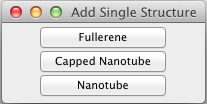
\includegraphics[scale= 0.6]{../../../../screens/nanocap_single_struct_win.png}
\caption{\nanocap~structure list for adding a single structure}
\label{f_single_structure_list}
\end{figure}
Adding a structures produces a blank \textit{template} containing no points or atoms. Each of the structures listed above are discussed in the following sections.

\subsection{Fullerenes}





The options to define the input parameters for the construction of the fullerene are displayed in the \textbf{Calculations--$>$Input} options:

 \begin{figure}[h!]
\centering
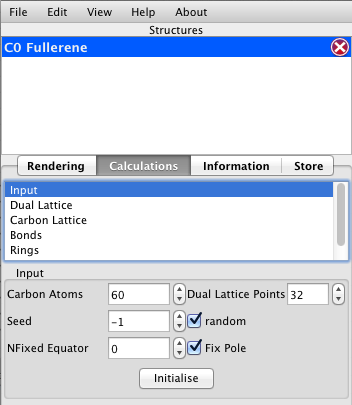
\includegraphics[scale= 0.6]{../../../../screens/nanocap_fullerene_input_win.png}
\caption{\nanocap~input options for a fullerene}
\label{fullerene_input_options}
\end{figure}

Here you can set the options for:
\begin{itemize}
 \item the number of dual lattice points or carbon atoms
 \item the seed for the initial random arrangement of dual lattice points
 \item the number of dual lattice points to hold fixed at either the poles or the equator
 \end{itemize}
 
Upon on clicking \textit{Initialise} the dual lattice points belonging to the fullerene will be constructed via the following:
\begin{equation}
\begin{array}{lcl}
x_i & = & \sqrt{1 - z_0}\cos(t_0) \\
y_i & = & \sqrt{1 - z_0}\sin(t_0) \\
z_i & = & z_0
\end{array}
\label{randomspheregen}
\end{equation}
where  $z_0$ and  $t_0$ are two random numbers in the range [$-$1,1] and [0,2$\pi$]. To visualise these points check the options outlined in Section \ref{Rendering}. The process of optimisation of these points is described in Section \ref{Optimisation}

%\documentclass{article}
%%\usepackage[html,png]{tex4ht}
%\usepackage{hyperref}
%
%\setlength\parindent{0pt}
%
%\title{Nanotubes}
%\date{}
%\begin{document}
%\maketitle

\subsection{Nanotubes}
%
%Although \nanocap~was designed to produce fullerenes and cap nanotubes, isolated nanotubes can be constructed. 
%
%A nanotube is constructed via:
%
%\textbf{File--$>$New Structure--$>$Single Structure}
%
%then click \textit{Nanotube} from the popup menu shown in Fig. ~\ref{n_single_structure_list}.
%
% \begin{figure}[h!]
%\centering
%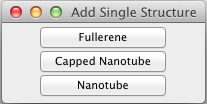
\includegraphics[scale= 0.6]{../../../../screens/nanocap_single_struct_win.png}
%\caption{\nanocap~structure list for adding a single structure}
%\label{n_single_structure_list}
%\end{figure}
%
%An unconstructed nanotube structure will then be added to the structure list:
%
%\begin{figure}[h!]
%\centering
%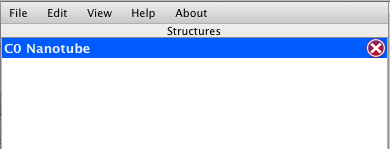
\includegraphics[scale= 0.6]{../../../../screens/nanocap_init_nanotube.png}
%\caption{\nanocap~structure list for adding a single structure}
%\label{init_nanotube}
%\end{figure}
%
%The template nanotube structure has no atoms or dual lattice points. 

To construct the carbon lattice the user has the option for either a finte-length nanotube or one that is periodic along the axial direction. 

 \begin{figure}[h!]
\centering
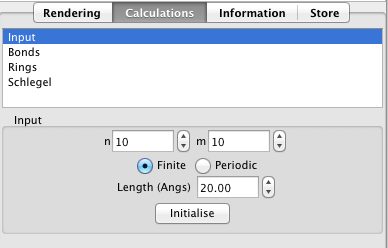
\includegraphics[scale= 0.5]{../../../../screens/nanocap_nanotube_init_finite_win.png}
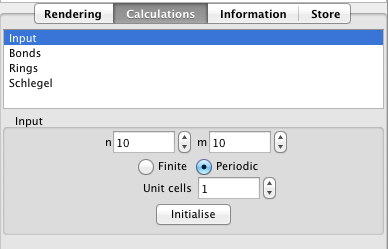
\includegraphics[scale= 0.5]{../../../../screens/nanocap_nanotube_init_periodic_win.png}
\caption{Nanotube construction options}
\label{nanotube_constructure_options}
\end{figure}

\subsubsection{Finite tubes}

Finite tubes are constructed as close to a user defined length as possible. This is done by constructing \textit{strips} of basis points along the chiral vector ($n,m$):

\begin{equation*}
\begin{array}{rl}
 \vect{P}_i  & =  n_i\vect{a_1} + m_i\vect{a_2}\\
 \vect{a_1}  &=  \tfrac{\sqrt{3}a_c}{2} (\sqrt{3}, 1)\\
 \vect{a_2}  &=  \tfrac{\sqrt{3}a_c}{2} (\sqrt{3}, -1)\\
\end{array}
\end{equation*}

\noindent where $a_c$ is the carbon bond length of 1.421~\AA. The incremented values ($n_i,m_i$) range from (0,0) to ($n,m$) and depends on:
\begin{equation*}
\begin{array}{rl}
n_i\verb!++! &\mbox{ if~~$m_i/( 2n_i+m_i)>m/( 2n+m)$} \\
m_i\verb!++! &\mbox{ if~~$m_i/( 2n_i+m_i)\leq m/( 2n+m)$} \\
 \end{array}
\end{equation*}
\noindent After each new row of points, the origin is translated in the $z$ direction by $\sqrt{3}a_c$. The current distance along the nanotube axis is then compared against the user defined length to determine if another strip should be added. The user defined length is inputted in the \textbf{Calculations--$>$Input} options.
 

At each basis point $\vect{P}$ at position $(p_x,p_z)$, the positions of the carbon atoms ($\vect{A}$ and  $\vect{B}$) and dual lattice points ($\vect{D}$) are given by:
\begin{equation*}
\begin{split}
\vect{A} &=  (p_x  , p_z)\\
\vect{B} &=  (p_x +a_c  , p_z)\\
 \vect{D} &=  (p_x + 2a_c , p_z)
 \end{split}
\end{equation*}

 
\subsubsection{Periodic tubes}

Periodic tubes are constructed using a user defined number of unit cells in the \textit{z} direction. The \textbf{periodic length}  $L$ of a nanotube of chirality ($n,m$) with $u$ unit cells is given by:

\begin{equation*}
\begin{split}
L &= u*|\vect{T}|\\
\vect{T}  &= t_1\vect{a_1} + t_2\vect{a_2}
 \end{split}
\end{equation*}
\noindent where the coefficients $t_1$ and $t_2$ have no common divisors except for unity and are given by:
\begin{equation*}
\begin{split}
 t_1 &= (2m + n)/ d_{R} \\
 t_2 &= -(2n + m)/ d_{R} \\
d_{R} &= \texttt{gcd}(2n+m, 2m+n)
 \end{split}
\end{equation*}

During construction the carbon atoms and dual lattice points are constructed as for the finite tubes with the replacement of the user-defined length with the periodic length. After construction, any points surpassing the periodic length are removed.

The number of unit cells can also be found in the \textbf{Calculations--$>$Input} options.

The \textbf{periodic length} can be found in the \textbf{Information} options tab. This will be required by simulation software if the nanotube is to be
used in a periodic simulation.

%\end{document}
%\documentclass{article}
%%\usepackage[html,png]{tex4ht}
%\usepackage{hyperref}
%\setlength\parindent{0pt}
%
%\title{Capped Nanotubes}
%\date{}
%\begin{document}
%\maketitle

\subsection{Capped Nanotubes}\label{cappednanotubes}

%The capped nanotube structure is the only structure that has associated child structures; a \textit{nanotube} and two \textit{cap} structures (labelled \textit{primary} and \textit{secondary}). The nanotube structure is the same class as that constructed during the isolated nanotube construction, apart from the nanotube always being of finite length. The cap structures can only be constructed as part of the parent capped nanotube structure.  
%
%As with the construction of fullerenes, capped nanotubes are either produced individually or by generating a series of structures for a given chirality and number of cap atoms.
%
%A single capped nanotube is constructed via:
%
%\textbf{File--$>$New Structure--$>$Single Structure}
%
%then click \textit{Capped Nanotube} from the popup menu shown in Fig. ~\ref{c_single_structure_list}.
% \begin{figure}[h!]
%\centering
%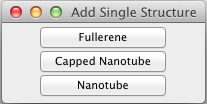
\includegraphics[scale= 0.6]{../../../../screens/nanocap_single_struct_win.png}
%\caption{\nanocap~structure list for adding a single structure}
%\label{c_single_structure_list}
%\end{figure}
%
%The capped nanotube structure added is a blank \textit{template} structure containing no points or atoms.  

The options to define the input parameters for the construction of the capped nanotube are displayed in the \textbf{Calculations--$>$Input} as shown in Fig~\ref{capped_nanotube_input_options}:

 \begin{figure}[h!]
\centering
\includegraphics[scale= 0.5]{../../../../screens/nanocap_capped_nanotube_input_win.png}
\caption{\nanocap~input options for a capped nanotube}
\label{capped_nanotube_input_options}
\end{figure}

The following input options can be set for the capped nanotube construction.
\begin{itemize}
 \item the chirality ($n,m$)
 \item the length of the nanotube (\AA)
 \item the number of cap carbon atoms and dual lattice points (or enabled the estimation based upon the nanotube density)
 \item the seed for the initial random cap point placement
 \item the force cutoff relating to the dual lattice force field (Section \ref{dforcefields})
 \end{itemize}
 
 
 

\section{Generating Multiple Structures}
\subsection{Structure Search}

As an alternative to constructing a single structure, \nanocap includes a tool for finding low energy structures by performing a \textit{structure search}. This is useful when finding the lowest energy topology is important or when an ensemble of structures are required. 

The structure search options are accessed through the \textbf{File--$>$New Structure--$>$Structure Search} menu. The structure search window includes a panel of parameters that define the structure type and search criteria. Here the user can define the required structural properties as well as the force field and optimiser to use during the search. The search results are dynamically displayed in a table where the user can browse the details of each structure. During the search the user can view an individual structure by pressing the \textbf{view} button in the associated row in the table. This will load the structure into the main \nanocap~window. An example of the structure search window during a search in shown in Fig.~\ref{structure_search_progress}

\begin{figure}[h!]
\centering
\includegraphics[scale= 0.4]{../../../../screens/nanocap_structure_search_progress.png}
\caption{\nanocap~structure search window during a search}
\label{structure_search_progress}
\end{figure}

After a structure search, the current set of results can be compared against the local and online (in future releases) databases. The columns in the structure search table denoted \textbf{Local} and \textbf{Web} indicate the presence of the structure in the associated databases. If a structure is not found it's icon will change (to a \textbf{+} symbol) and it can be immediately added to the corresponding database with a single click. Results from a typical structure search after checking against the local \nanocap~database are shown in Fig.~\ref{structure_search_check}

 \begin{figure}[h!]
\centering
\includegraphics[scale= 0.4]{../../../../screens/nanocap_structure_search_check.png}
\caption{\nanocap~structure search window after a search and results have been checked against the local database}
\label{structure_search_check}
\end{figure}

\section{Force Fields}\label{forcefields}

\nanocap~implements force fields for the optimisation of the both the dual lattices and carbon lattices of each structure. When a structure is saved information relating to the force field is also stored. This allows the same topologies to be optimised by various force fields. Outlined in the next sections are the force fields currently available in \nanocap~.

\subsection{Dual Lattice Force Fields}\label{dforcefields}

Currently, only one force field is implemented to optimise a structure's dual lattice - labelled: \textit{The Thomson Problem}. The total energy of a system of $N_D$ dual lattice points is given by the sum of pair interaction energies:

\begin{equation*}
 \displaystyle \phi = \sum_{i=1}^{N_{D}}\sum_{j=i+1}^{N_{D}}\frac{1}{| \vect{r_i}-\vect{r_j}| } 
\end{equation*}

where $\vect{r}$ denotes the position vector of each point. When the dual lattice belongs to a fullerene, the full system is included in the loop of pair interactions. For a capped nanotube however, there is restriction to the points included in the force field calculation. A cutoff length is introduced along the nanotube beyond which points are exclude from the force evaluation. This is required to ensure a uniform arrangement of points in the capped region and reduce the concentration of points in the apex of the cap. This cutoff length is automatically determined basen upon the density of points in the nanotube but can be set manually in the options described in Section \ref{cappednanotubes}

\subsection{Carbon Lattice Force Fields}

Currently there are 3 force fields implemented in \nanocap. These are selected in the \textbf{Calculations--$>$Carbon Lattice} options as shown in Fig.~\ref{carbonlatticeoptions}.

 \begin{figure}[h!]
\centering
\includegraphics[scale= 0.6]{../../../../screens/nanocap_carbon_lattice_options_win.png}
\caption{\nanocap~input options for a fullerene}
\label{carbonlatticeoptions}
\end{figure}

Each force field is described below:

 \begin{enumerate}
 
\item \textbf{Unit Radius Topology} 

By default, when a carbon lattice is constructed a carbon force field is not used and the structure is simply a result of the triangulated dual lattice. This generates a topology of unit radius (cylindrical if a capped nanotube) and as such is labelled the 

\item \textbf{Scaled Topology} 

The simplest force field that produces a carbon structure of physical dimensions is the \textbf{scaled topology} force field. This forcefield uses the ideal C-C bond length of 1.421 \AA~ to optimise the carbon lattice. The fictitious \textit{energy} is given by the sum of squares deviation from this ideal bond length. This force field only does return derivatives and as such can only be used with the \textbf{MC} or \textbf{SIMPLEX} optimisers (see Section \ref{Optimisation}).

\item \textbf{EDIP}

The most sophistic force field implemented in \nanocap~is the Environmental Dependence Interatomic Potential (EDIP). Using EDIP produces the most physically sound structures and its use is recommended. For a theoretical description of EDIP please refer to the following paper: 

\textbf{Generalizing the environment-dependent interaction potential for carbon}

N. A. Marks \textit{Phys. Rev. B 63, 035401 2000}

url: \url{http://journals.aps.org/prb/abstract/10.1103/PhysRevB.63.035401}

  
 \end{enumerate}
%\end{document}


    

\section{Optimisation}\label{Optimisation}

The underlying design of \nanocap~ and the generalisation of point sets and forcefields, allows for a great deal of flexibility in optimisation routines. The same optimisation routine that is used to minimised the total dual lattice energy can be used to optimise the carbon lattice using a force field such as EDIP. Currently three methods of minimising the total energy are implemented and can be selected in either the  \textbf{Calculations--$>$Dual Lattice} or  \textbf{Calculations--$>$Carbon Lattice} options as shown in Fig.~\ref{optimisation_options}

 \begin{figure}[h!]
\centering
\includegraphics[scale= 0.5]{../../../../screens/nanocap_dual_lattice_options_win.png}
\includegraphics[scale= 0.5]{../../../../screens/nanocap_carbon_lattice_options_win.png}
\caption{\nanocap~Optimisation options are shown for both the dual lattice and carbon lattice option windows.}
\label{optimisation_options}
\end{figure}

These options include the number of minimisation steps and the tolerance used to determine convergence. A brief description of each of the optimisers is given below:

 \begin{enumerate}

\item \textbf{L-BFGS}

The tastes, most robust optimiser is the Limited-memory Broyden--Fletcher--Goldfarb--Shanno method (LBFGS). This routine requires forces which are used to iteratively update an estimate of the Hessian matrix, which in turn is used to define new directions along which to perform line searches. \nanocap~uses the the LBFGS method as implemented in the \texttt{scipy.optimise} libraries (\url{http://docs.scipy.org/doc/scipy/reference/generated/scipy.optimize.fmin_l_bfgs_b.html}). 


\textbf{A Limited Memory Algorithm for Bound Constrained Optimization} R. H. Byrd, P. Lu and J. Nocedal.  \textit{(1995), SIAM Journal on Scientific and Statistical Computing, 16, 5, pp. 1190-1208.}

\textbf{L-BFGS-B: Algorithm 778: L-BFGS-B, FORTRAN routines for large scale bound constrained optimization} C. Zhu, R. H. Byrd and J. Nocedal.  \textit{(1997), ACM Transactions on Mathematical Software, 23, 4, pp. 550 - 560.}

\textbf{L-BFGS-B: Remark on Algorithm 778: L-BFGS-B, FORTRAN routines for large scale bound constrained optimization} J.L. Morales and J. Nocedal.  \textit{ (2011), ACM Transactions on Mathematical Software, 38, 1.}

\item \textbf{SD}

The steepest descent (SD) method minimises energy by simply following the direction of force (or the negative gradient of the potential field). The step size per iteration is determined by the current magnitude of force. The SD method is useful when visualising the optimisation process.

\item \textbf{SIMPLEX}

The simplex method is an optimisation routine which does not require the calculation of forces. As such is the only optimiser that works with the \textbf{Scaled Topology} force field. The implementation in \nanocap~again comes from the \texttt{scipy.optimise} libraries which implement algorithms presented in the following publications:

\textbf{A Simplex Method for Function Minimization} Nelder, J.A. and Mead, R. \textit{The Computer Journal, 7, pp. 308-313}

\textbf{Direct Search Methods: Once Scorned, Now Respectable} Wright, M.H.  \textit{Numerical Analysis 1995, Proceedings of the 1995 Dundee Biennial Conference in Numerical Analysis pp. 191-208}


 \end{enumerate}

\section{Storing, Loading and Exporting}

Each individual structure loaded or created can be checked against the local and online \nanocap~databases. This is carried out in the \textbf{Storage} window on the main toolbar as shown in Fig.~\ref{StoreOptions}. 

 \begin{figure}[h!]
\centering
\includegraphics[scale= 0.6]{../../../../screens/nanocap_single_storage.png}
\caption{Checking a structure against the local and online \nanocap~databases}
\label{StoreOptions}
\end{figure}


\subsection{The Local NanoCap Database}

One of the main features of \nanocap~is the local database of structures which allows the user to efficiently store previously generated structures. By default the database is stored in the \nanocap~user directory (.nanocap). The database can be accessed in several ways; using the \nanocap~GUI, using the \nanocap~scripts or using an external SQLite client. Using the GUI,the \textbf{Database Viewer} window is located in the  \textbf{View--$>$Local Database} menu. 

 \begin{figure}[h!]
\centering
\includegraphics[scale= 0.6]{../../../../screens/nanocap_db_menu.png}
\includegraphics[scale= 0.6]{../../../../screens/nanocap_db_viewer.png}
\caption{\nanocap~database viewer}
\label{DBViewer}
\end{figure}

The database viewer provides an interactive interface to the \nanocap~database allowing real time searching and loading of stored structures (Fig.~\ref{DBViewer}). Additional search parameters can be added by pressing the \textbf{Select Properties} button which displays all possible database fields. When searching for a structure, logical expressions can be used for each file. For example, if \lq\texttt{> 100}\rq~is entered into the \texttt{Natoms} fields then only structures with more than 100 atoms will be returned. The column labelled \lq\texttt{>View}\rq~ provides buttons to load a structure into the main \nanocap~window. The loaded structures can then be modified, for example re-optimised with a different force field.

To access the database via \python~scripts, the \nanocap~libraries can be used. For examples of these scripts see Section~\ref{Examples}.

As the \nanocap~database is written using SQLite, a suitable database client can be used to view the database. An example using the \texttt{sqlite3} client is shown below: 

\begin{lstlisting}[keywordstyle={\color{myterminalfont}},
			language={sh},
			commentstyle={\it\color{myterminalfont}},
			emphstyle={\ttb\color{myterminalfont}},
			stringstyle={\color{myterminalfont}},
			showstringspaces={false},
			otherkeywords={self},
			emph={MyClass,__init__},
			frame={},
			basicstyle={\ttm\color{myterminalfont}},
			morekeywords={True,False},
			captionpos={b},
			backgroundcolor={\color{myterminalbg}}]		
bash-3.2$ sqlite3 ~/.nanocap/nanocap.db
SQLite version 3.7.13 2012-06-11 02:05:22
Enter ".help" for instructions
Enter SQL statements terminated with a ";"
sqlite> .headers on;
sqlite> .mode column
sqlite> select id,type,Natoms,energy,ff_id from carbon_lattices
   ...> where type="Fullerene" and ff_id="EDIP";
id          type        natoms      energy            ff_id               
----------  ----------  --------  ----------------  --------------------
11          Fullerene   220       -1550.4155355469  EDIP                   
50          Fullerene   200       -1403.7245939477  EDIP                
51          Fullerene   200       -1403.5958295534  EDIP                
52          Fullerene   200       -1404.0657391286  EDIP                
53          Fullerene   200       -1402.8514086776  EDIP                
54          Fullerene   200       -1403.3230258698  EDIP                
55          Fullerene   200       -1404.3263445713  EDIP                
56          Fullerene   200       -1403.4800906205  EDIP                
57          Fullerene   200       -1404.3965982273  EDIP                
58          Fullerene   200       -1404.1298467551  EDIP                
59          Fullerene   200       -1403.4657122674  EDIP                
64          Fullerene   200       -1403.7245939160  EDIP
\end{lstlisting}


\subsection{The Online NanoCap Database}

The online \nanocap~database is currently under construction.

\subsection{Exporting}

Each structure in the current structure list can be exported to file. The options for exporting a structure can be found in the \textbf{File--$>$Export Structure} menu. The full list of export options are shown in Fig.~\ref{export_struct_optionst}. 


 \begin{figure}[hp]
\centering
\includegraphics[scale= 0.6]{../../../../screens/nanocap_export_structure_menu.png}
\includegraphics[scale= 0.6]{../../../../screens/nanocap_export_structure_win.png}
\caption{\nanocap~export structure options}
\label{export_struct_optionst}
\end{figure}

The export options include the ability to select which lattices are saved and in what file format. Currently only a simple $xyz$ file format is implemented which contains a minimum amount of data (the number of points and positions). In addition to the topology of the structure, structural information can also be saved. This includes energies, dimensions, connectivity (ring statistics) amongst other things.Using the rendering capabilities of \nanocap, images of the structure can also be automatically saved. This includes a series of images that capture a full rotation of the structure. These images can be encoded into a movie to simplify future inspection of the stored structure. Finally, the export options require a parent directly to save the aforementioned data. Within this directory a new directory will be created whose name uniquely identifies the current structure.

\section{Rendering}\label{Rendering}

\nanocap~provides a 3D rendering and interaction interface using the \texttt{VTK} libraries and the associated widgets in \texttt{Qt}. This allows real time inspection of the structures that are being constructed or previously found structures loaded from the database. Current capabilities include the rendering of both dual and carbon lattices, the carbon-carbon bonds, the ring network and the dimensions of the current structure. These options are dynamics, with any changes to the appearance of the current structure changing in real time. An example of the \nanocap rendering options and render window are shown in Fig.~\ref{renderingwindow}.

 \begin{figure}[hp]
\centering
\includegraphics[scale= 0.45]{../../../../screens/nanocap_rendering_window.png}
\caption{The \nanocap~rendering options and the corresponding render window.}
\label{renderingwindow}
\end{figure}

\subsection{Schlegel View}

In addition to the 3D view of the current structure a 2D projection (Schlegel) view can also be rendered. The two parameters involved in the calculation of this projection are accessed through \textbf{Calculations--$>$Schlegel}. The parameter \texttt{Gamma}($\gamma$) determines the magnitude of the projection via:
\begin{equation*}
\begin{split}
\vect{r'} &= (x_i,y_i)\\
x' &= x + \gamma_s\cdot \frac{x}{|\vect{r'}|} \\
y' &= y + \gamma_s\cdot \frac{y}{|\vect{r'}|} \\
\end{split}
\end{equation*}
The \texttt{Cutoff} value determines the points that are used for the projection. An example projection is shown in Fig.~\ref{schlegelrenderingwindow}.

 \begin{figure}[hp]
\centering
\includegraphics[scale= 0.45]{../../../../screens/nanocap_schlegel_options.png}
\includegraphics[scale= 0.45]{../../../../screens/nanocap_schlegel_window.png}
\caption{Schlegel options and render window.}
\label{schlegelrenderingwindow}
\end{figure}



%\documentclass{article}
%\usepackage[html,png]{tex4ht}
%\usepackage{hyperref}
%\setlength\parindent{0pt}
%
%\title{Documentation}
%\date{}
%\begin{document}
%\maketitle

\section{Scientific Publications}

There are two papers associated with the theory and implementation of \nanocap. If \nanocap~is used in your work, please cite the following:

\begin{enumerate}
\item \textbf{Generalized method for constructing the atomic coordinates of nanotube caps}

M. Robinson, I. Suarez-Martinez, and N. A. Marks \textit{Phys. Rev. B 87, 155430 2013}

Abstract:

A practical numerical method for the rapid construction of nanotube caps is proposed. 
Founded upon the notion of lattice duality, the algorithm considers the face dual representation of a given nanotube which is used to solve an energy minimization problem analogous to The Thomson Problem. 
Not only does this produce caps for nanotubes of arbitrary chirality, but the caps generated will be physically sensible and in most cases the lowest energy structure. 
To demonstrate the applicability of the technique, caps of the (5,5) and the (10,0) nanotubes are investigated by means of density-functional tight binding (DFTB). 
The calculation of cap energies highlights the ability of the algorithm to produce lowest energy caps. 
Due to the preferential construction of spherical caps, the technique is particularly well suited for the construction of capped multiwall nanotubes (MWNTs). To validate this proposal and the overall robustness of the algorithm, a MWNT is constructed containing the chiralities (9,2)@(15,6)@(16,16). 
The algorithm presented paves the way for future computational investigations into the physics and chemistry of capped nanotubes.

%url: http://journals.aps.org/prb/abstract/10.1103/PhysRevB.87.155430

url: \href{http://journals.aps.org/prb/abstract/10.1103/PhysRevB.87.155430}{\texttt{http://journals.aps.org/prb/abstract/10.1103/PhysRevB.87.155430}}
%url: \url{ http://journals.aps.org/prb/abstract/10.1103/PhysRevB.87.155430}%{ http://journals.aps.org/prb/abstract/10.1103/PhysRevB.87.155430}

\item \textbf{NanoCap: A Framework for Generating Capped Carbon Nanotubes and Fullerenes}

M. Robinson and N. A. Marks \textit{Com. Phys. Comm 2014}

Abstract:

NanoCap provides both libraries and a standalone application for the construction of capped nanotubes of arbitrarily chirality and fullerenes of any radius. 
Structures are generated by constructing a set of optimal dual graph topologies which are subsequently optimised using a carbon interatomic potential. 
Combining this approach with a GUI featuring 3D rendering capabilities allows for the rapid inspection of physically sensible structures which can be used as input for molecular simulation.

url: *tba*

\end{enumerate}

%\end{document}


\section{Code}\label{Code}

\subsection{Non-GUI Class Structure}

The basic class structure of the non-GUI elements of \nanocap~are is shown in Fig.~\ref{ClassUML}.  The class diagrams are constructed with the help of \texttt{pyreverse} and \texttt{graphviz}.

%\begin{landscape}
 \begin{figure}[!h]
\centering
\includegraphics[width=18cm, angle =90]{../../../../uml/nanocap_class_UML.png}
\caption{Class diagram of the non GUI classes in \nanocap.}
\label{ClassUML}
\end{figure}
%\end{landscape}

\subsection{GUI Class Structure}

The main GUI elements are shown in the class diagram in Fig.~\ref{ClassUMLgui}.

 \begin{figure}[!h]
\centering
\includegraphics[width=22cm, angle =90]{../../../../uml/nanocap_class_gui_UML.png}
\caption{Class diagram of the GUI classes in \nanocap.}
\label{ClassUMLgui}
\end{figure}
\section{Examples}\label{Examples}

The following section lists example scripts that utilise the \nanocap~libraries. %The current example list is as follows:

%\begin{itemize}
% \item \verb|nanocap_nanotube.py| 
% \item \verb|nanocap_single_fullerene.py| 
% \item \verb|nanocap_bulk_fullerenes.py| 
%  \item \verb|nanocap_bulk_fullerenes.py| 
%   \item \verb|nanocap_bulk_fullerenes.py| 
%   
% \end{itemize}

These examples can be found in the \texttt{example\_scripts} directory of the \nanocap~source.


\subsection{Nanotube Construction}

\verb|nanocap_nanotube.py| an example script to construct an uncapped nanotube. The code is shown below.

\lstinputlisting[keywordstyle={\ttb\color{blue}},
			language={Python},
			commentstyle={\tti\color{mygreen}},
			emphstyle={\ttb\color{deepred}},
			stringstyle={\color{deepgreen}},
			showstringspaces={false},
			otherkeywords={self},
			emph={MyClass,__init__},%,nanocap,structures,nanocap,core},
			frame={single},
			basicstyle={\ttm\color{black}},
			morekeywords={True,False},
			captionpos={b},
			backgroundcolor={\color{mycodebg}},
			rulecolor={\color{mycodeborder}}]%
			{../../example_scripts/nanocap_nanotube.py}

\subsection{Fullerenes}

\subsubsection{Single Fullerene Construction}

\verb|nanocap_single_fullerene.py| is an example script to construct and save a fullerene. The code is shown below.

\lstinputlisting[keywordstyle={\ttb\color{blue}},
			language={Python},
			commentstyle={\tti\color{mygreen}},
			emphstyle={\ttb\color{deepred}},
			stringstyle={\color{deepgreen}},
			showstringspaces={false},
			otherkeywords={self},
			emph={MyClass,__init__},%,nanocap,structures,nanocap,core},
			frame={single},
			basicstyle={\ttm\color{black}},
			morekeywords={True,False},
			captionpos={b},
			backgroundcolor={\color{mycodebg}},
			rulecolor={\color{mycodeborder}}]%
			{../../example_scripts/nanocap_single_fullerene.py}

\subsubsection{Constructing Multiple Fullerenes }

\verb|nanocap_bulk_fullerenes.py| is an example script to perform a structure search to construct and save multiple fullerenes. The code is shown below.

\lstinputlisting[keywordstyle={\ttb\color{blue}},
			language={Python},
			commentstyle={\tti\color{mygreen}},
			emphstyle={\ttb\color{deepred}},
			stringstyle={\color{deepgreen}},
			showstringspaces={false},
			otherkeywords={self},
			emph={MyClass,__init__},%,nanocap,structures,nanocap,core},
			frame={single},
			basicstyle={\ttm\color{black}},
			morekeywords={True,False},
			captionpos={b},
			backgroundcolor={\color{mycodebg}},
			rulecolor={\color{mycodeborder}}]%
			{../../example_scripts/nanocap_bulk_fullerenes.py}

\subsection{Capped Nanotube Construction}

\subsubsection{Single Capped Nanotube Construction}

\verb|nanocap_single_capped_nanotube.py| is an example script to construct and save a capped nanotube. The code is shown below.

\lstinputlisting[keywordstyle={\ttb\color{blue}},
			language={Python},
			commentstyle={\tti\color{mygreen}},
			emphstyle={\ttb\color{deepred}},
			stringstyle={\color{deepgreen}},
			showstringspaces={false},
			otherkeywords={self},
			emph={MyClass,__init__},%,nanocap,structures,nanocap,core},
			frame={single},
			basicstyle={\ttm\color{black}},
			morekeywords={True,False},
			captionpos={b},
			backgroundcolor={\color{mycodebg}},
			rulecolor={\color{mycodeborder}}]%
			{../../example_scripts/nanocap_single_capped_nanotube.py}

\subsubsection{Constructing Multiple Capped Nanotubes }

\verb|nanocap_bulk_capped_nanotubes.py| is an example script to perform a structure search to construct and save multiple capped nanotube. The code is shown below.

\lstinputlisting[keywordstyle={\ttb\color{blue}},
			language={Python},
			commentstyle={\tti\color{mygreen}},
			emphstyle={\ttb\color{deepred}},
			stringstyle={\color{deepgreen}},
			showstringspaces={false},
			otherkeywords={self},
			emph={MyClass,__init__},%,nanocap,structures,nanocap,core},
			frame={single},
			basicstyle={\ttm\color{black}},
			morekeywords={True,False},
			captionpos={b},
			backgroundcolor={\color{mycodebg}},
			rulecolor={\color{mycodeborder}}]%
			{../../example_scripts/nanocap_bulk_capped_nanotubes.py}
			
\subsection{Database Operations}

As \nanocap~uses an sqlite database, the database can be browsed from the command line:


\subsubsection{Saving structures to the local database }

\verb|nanocap_add_structure_to_db.py| is an example script to save a fullerene structure to disk. The code is shown below.

\lstinputlisting[keywordstyle={\ttb\color{blue}},
			language={Python},
			commentstyle={\tti\color{mygreen}},
			emphstyle={\ttb\color{deepred}},
			stringstyle={\color{deepgreen}},
			showstringspaces={false},
			otherkeywords={self},
			emph={MyClass,__init__},%,nanocap,structures,nanocap,core},
			frame={single},
			basicstyle={\ttm\color{black}},
			morekeywords={True,False},
			captionpos={b},
			backgroundcolor={\color{mycodebg}},
			rulecolor={\color{mycodeborder}}]%
			{../../example_scripts/nanocap_add_structure_to_db.py}

\subsubsection{Loading structures from the local database }

\verb|nanocap_load_from_db.py| is an example script to load a set of fullerene dual lattices and save to disk. The code is shown below.

\lstinputlisting[keywordstyle={\ttb\color{blue}},
			language={Python},
			commentstyle={\tti\color{mygreen}},
			emphstyle={\ttb\color{deepred}},
			stringstyle={\color{deepgreen}},
			showstringspaces={false},
			otherkeywords={self},
			emph={MyClass,__init__},%,nanocap,structures,nanocap,core},
			frame={single},
			basicstyle={\ttm\color{black}},
			morekeywords={True,False},
			captionpos={b},
			backgroundcolor={\color{mycodebg}},
			rulecolor={\color{mycodeborder}}]%
			{../../example_scripts/nanocap_load_from_db.py}



\end{document}